\section{The Lean Startup}
\label{sec:LeanStartup}
\ac{TLS} beschreibt eine Sammlung an Konzepten, welche sich, nach \citeA{TheLeanStartup}, bei der Gründung von Startups als erfolgreich erwiesen haben. Der \ac{TLS}-Ansatz besteht aus unterschiedlichen Methoden, welche häufigen Fehlern im Umgang mit Startups entgegenwirken sollen, um diese Firmen vor dem Scheitern zu bewahren.

Der Autor grenzt ein Startup mit einer eigenen Definition der Unternehmensform klar von etablierten Firmen ab:
\begin{quote}
,,A human institution designed to create new products and services under conditions of extreme uncertainty.'' \cite[S. 8]{TheLeanStartup}
\end{quote}
Das Schlüsselwort \textit{uncertainty} - zu deutsch: Unsicherheit - in diesem Satz ist essentiell, da eine große Herausforderung eines Startups darin besteht, ein Produkt zu entwickeln, welches den Endnutzern einen Vorteil bietet. Im Gegensatz zu etablierten Unternehmen, welche bereits viele Erfahrungen mit dem Verhalten der Kunden haben, sind die Wünsche und Bedürfnisse der Kunden für ein Startup vorerst unbekannt. Daher entstehen Vermutungen über das Verhalten der Zielgruppe, welche meist nicht belegt werden können. Durch unbeweisbare Annahmen ensteht diese Unsicherheit. Deshalb ist das Hauptziel des \ac{TLS}-Modells, diese zu minimieren indem sämtliche Hypothesen über die Wünsche und Bedürfnisse der potentiellen Kunden im Rahmen von Tests geprüft werden. Dadurch können sichere Rückschlüsse gezogen werden, was wiederum das Gesamtrisiko minimiert.

Die genannten Konzepte werden im Folgenden genauer erläutert.

\subsection*{\refstepcounter{subsection}\label{sec:LeanStartup-ValidatedLearning}\thesubsection\quad Validated Learning}
Bei Startups entsteht oft das Problem, dass Erfolg zu Beginn nicht nach traditionellen Methoden gemessen werden kann. In einem etablierten Unternehmen gibt es für ein Projekt exakte Zeit- und Budgetvorgaben, welche einzuhalten sind. Ist dies gelungen, gilt das Projekt als erfolgreich. Wendet man diese Methode bei einem Startup an, ist es möglich, dass diese Vorgaben zwar eingehalten werden, jedoch wird das Produkt nicht verkauft, da es keine Nachfrage dafür gibt. In diesem Fall war das Projekt nach klassischem Denken erfolgreich, das Produkt allerdings nicht. Nach der gesamten Projektlaufzeit hat das Unternehmen dabei gelernt, dass das Produkt geändert werden muss. \citeauthor{TheLeanStartup} erklärt, dass dieses Wissen bereits in einer kürzeren Zeitspanne erlangt werden kann. Dafür entwickelt er eine Herangehensweise, welche \ac{VL} genannt wird. Diese wurde entwickelt, um Fortschritt im Sinne von Wissen über die Zielgruppe nachzuweisen und zu demonstrieren. Im Gegensatz zu klassischen Prognosen über den Markt und Produkterfolg werden mit Hilfe von \ac{VL} im Rahmen von empirischen Beobachtungen nachweisbare Ergebnisse erbracht. Das Grundprinzip besteht darin, grundsätzliche Annahmen über den Endnutzer und das Produkt in kleineren Experimenten zu testen. Das heißt, sämtliche Vermutungen über die Wünsche oder Bedürfnisse der Zielgruppe werden im Rahmen der \ac{BML} Schleife, welche in Abschnitt \ref{sec:LeanStartup-BML} genauer erklärt wird, geprüft. Damit kann die Richtigkeit dieser Annahmen im Vorfeld gesichert werden. So können bereits im frühen Stadium der Entwicklung viele Risiken eliminiert werden, da das Verhalten der Nutzer von Anfang an getestet anstatt abgeschätzt wird.

Durch diese empirischen Daten kann ein Startup viele messbare Einblicke über die Zielgruppe hervorbringen. Je genauer die Wünsche und Bedürfnisse der Endkunden bekannt sind, desto einfacher ist es im Umkehrschluss, ein auf die Nutzer abgestimmtes Produkt zu entwickeln. Daher stellt jeder Einblick eine eigene Einheit für Fortschritt dar, erklärt \citeauthor{TheLeanStartup}.

\subsection*{\refstepcounter{subsection}\label{sec:LeanStartup-BML}\thesubsection\quad Bauen-Messen-Lernen}
\begin{figure}
	\begin{center}
		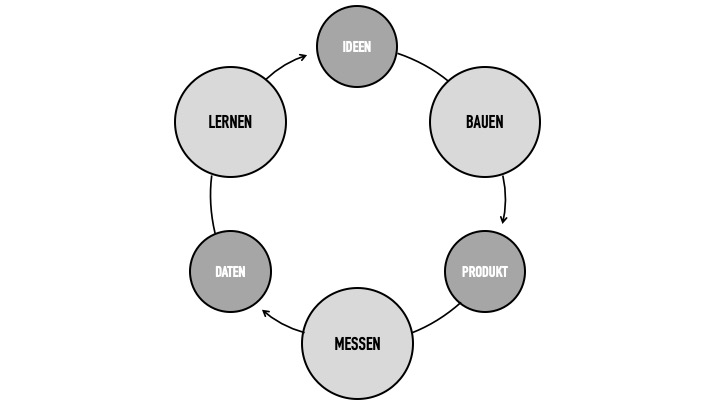
\includegraphics[scale=0.5]{99_IMG/02_Grundlagen/buildmeasurelearn.jpg}
		\caption[Modell der \ac{BML} Schleife nach dem \ac{TLS}-Konzept.]{Modell der \ac{BML} Schleife nach dem \ac{TLS}-Konzept (Abbildung übersetzt aus \citeNP{TheLeanStartup}).}
		\label{fig:LeanStartup_BuildMeasureLearn}
	\end{center}
\end{figure}
Wie in Abb. \ref{fig:LeanStartup_BuildMeasureLearn} dargestellt, beschreibt dies eine Abfolge von Aufgaben, die maximalen Lerneffekt versprechen. Diese wird oft wiederholt, um neue Einsichten zu gewinnen. Daher entsteht pro Iteration ein neuer Lerneffekt, da bei jedem Durchlauf ein anderer Baustein getestet wird. Um diese Details zu definieren, wird die Schleife rückwärts geplant. Erst muss festgelegt werden, welche Einblicke in dieser Iteration wichtig sind bzw. was genau im Rahmen dieser Iteration herausgefunden werden soll. Mit dieser Grundlage wird dann beschlossen, welche Messungen nötig sind, um die richtigen und eindeutigen Einblicke zu bekommen. Danach kann erst entschieden werden, was dafür gebaut werden muss. Dabei kann es sich um einzelne Zusatzfunktionen handeln, aber auch um ein komplettes Produkt. Bei einem neuen Produkt ist es wichtig, nur die Schlüsselfunktionen zu entwickeln, also den Kern des Endproduktes. Darunter versteht man auch ein \textit{\ac{MVP}}. Das ist eine Version des Produktes, welche einen kompletten Durchlauf der Schleife bei minimaler Entwicklungszeit ermöglicht. Dabei ist es plausibel, dass unnötige Details weggelassen werden müssen, da diese den Aufwand erhöhen würden, ohne einen Mehrwert nach sich zu ziehen.

\subsection*{\refstepcounter{subsection}\label{sec:LeanStartup-InnovationAccounting}\thesubsection\quad Innovation Accounting}
Die \textit{Innovation Accounting}-Methode ermöglicht es Startups, anhand von objektiven Beobachtungen und messbaren Erfolgen ein erfolgreiches Unternehmen aufzubauen, so \citeauthor{TheLeanStartup}. Zuerst wird ein \ac{MVP} entwickelt und getestet, um den Ausgangszustand des Startups einzuschätzen. Davon ausgehend wird die \ac{BML}-Schleife so oft durchlaufen, bis alle Annahmen über den Nutzer getestet und validiert sind. Schritt für Schritt entwickelt sich hier das Anfangsprodukt zu dem auf die Zielgruppe zugeschnittenen idealen Produkt. Solange das Unternehmen Fortschritte macht, gute Einblicke in die Kundensicht erhält und diese effektiv umsetzt, bewegt sich das Unternehmen weiter in Richtung Ideal. Ist das nicht der Fall, ist es unter Umständen Zeit für ein \textit{Pivot}, eine Methode, welche in Abschnitt \ref{sec:LeanStartup-Pivot} behandelt wird.

\subsection*{\refstepcounter{subsection}\label{sec:LeanStartup-Pivot}\thesubsection\quad Pivot}
\begin{figure}
	\begin{center}
		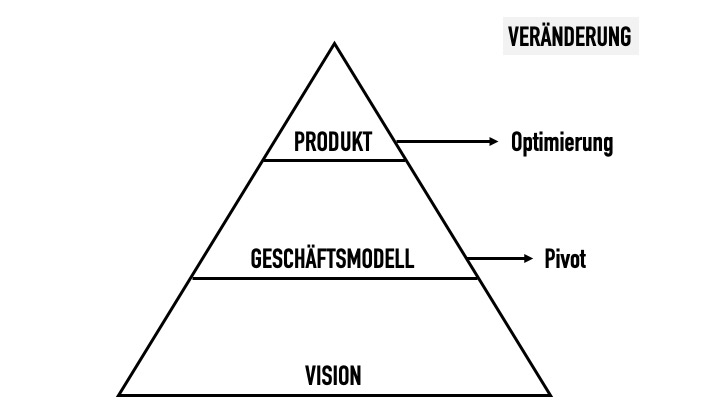
\includegraphics[scale=0.5]{99_IMG/02_Grundlagen/visionStrategyProduct.jpg}
		\caption[Unterteilung eines Projektes im \ac{TLS}-Modell.]{Unterteilung eines Projektes im \ac{TLS}-Modell (Abbildung übersetzt aus \citeNP{TheLeanStartup}).}
		\label{fig:LeanStartup_VisionStrategyProduct}
	\end{center}
\end{figure}
Unter einem \textit{Pivot} versteht man im Allgemeinen eine Kurskorrektur oder Abänderung des Geschäftsmodells. Nach \citeauthor{TheLeanStartup} ist jedes Startup-Projekt in drei Bausteine aufgeteilt. Diese werden Vision, Geschäftsmodell und Produkt genannt. Der Aufbau dieser Teile ist in der Abbildung \ref{fig:LeanStartup_VisionStrategyProduct} dargestellt. 
Die Vision liegt jeder Idee zugrunde. Sie beschreibt das Ziel, welches durch das Projekt auf lange Sicht erreicht werden soll. Die Vision selbst wird selten geändert, da sie der Grundbaustein des gesamten Startups ist. Darauf aufbauend entwickelt sich ein Geschäftsmodell nach dem das Produkt im Wesentlichen entwickelt wird. Die wichtigste und zugleich schwierigste Aufgabe eines Gründers ist zu entscheiden, wann sich das Geschäftsmodell des Projektes ändern muss. Der Autor empfiehlt dafür am Ende jeder \ac{BML}-Iteration ein \textit{Pivot}-Meeting einzuberufen. In diesem wird besprochen, ob das Experiment erfolgreich war oder nicht. Falls nicht, muss entschieden werden, ob das negative Ergebnis dem Geschäftsmodell geschuldet ist oder dem Produkt. Wie in Abb. \ref{fig:LeanStartup_VisionStrategyProduct} dargestellt, liegt der Unterschied darin, dass entweder ein \textit{Pivot} oder eine Feinabstimmung stattfinden muss. Dafür stellt \citeauthor{TheLeanStartup} unterschiedliche \textit{Pivot}-Modelle dar:
\begin{itemize}
	\item \textbf{Zoom-in Pivot:} Das neue Produkt besteht aus einem einzelnen Baustein des ursprünglich geplanten Produktes.
	\item \textbf{Zoom-out Pivot:} Das neue Produkt enthält das ursprünglich geplante Produkt als Feature.
	\item \textbf{Customer Segment Pivot:} Das Produkt wird auf eine andere Zielgruppe, als ursprünglich geplant, zugeschnitten.
	\item \textbf{Customer Need Pivot:} Das Produkt wird dahingehend abgeändert, dass ein unterschiedliches Problem der gleichen Zielgruppe damit gelöst wird. Das heißt, es stellt sich heraus, dass die Nutzer, mit denen zusammengearbeitet wird, andere Bedürfnisse haben, als ursprünglich angenommen.
	\item \textbf{Platform Pivot:} Software, welche ursprünglich als App geplant wurde, wird als Plattform realisiert oder umgekehrt.
	\item \textbf{Business Architecture Pivot:} Dieser Pivot beinhaltet den Wechsel vom B2B zum B2C Geschäft und umgekehrt.
	\item \textbf{Value Capture Pivot:} Die Art, durch welche das Produkt einen Wert für den Kunden erzeugt, wird geändert. 
	\item \textbf{Engine of Growth Pivot:} Der Erfolg des Produktes wird durch eine andere Methode gemessen. Die unterschiedlichen \textit{Engines of Growth} werden in Kapitel \ref{sec:LeanStartup-EnginesOfGrowth} erklärt.
	\item \textbf{Channel Pivot:} Der Vetriebskanal wird geändert. So wird das Produkt auf einem anderen Weg, als ursprünglich geplant, an den Kunden gebracht.
	\item \textbf{Technology Pivot:} Das Produkt wird auf technischer Ebene abgeändert. Das soll bessere Preisangebote oder Performance mit sich ziehen.
\end{itemize}
Ein Geschäftsmodell während der Entwicklung abzuändern, stellt eine große Schwierigkeit dar. Da es keine optimale Strategie für die Produktentwicklung gibt, muss jedes Startup ein eigenes Modell entwickeln, um maximalen Erfolg zu erzielen. Daher ist die Entschiedung, ein \textit{Pivot} durchzuführen, subjektiv und nicht messbar. Außerdem gibt es keine Garantie für den Erfolg des neuen oder abgeänderten Konzeptes. 

Das Geschäftsmodell ist wiederum das Fundament für das Endprodukt. Dies soll nach jeder Iteration abgewandelt werden, um den Wünschen und Bedürfnissen der Endkunden gerecht zu werden. Diese Änderungen werden demnach als Optimierung bezeichnet, da es sich um kleinere Anpassungen des Produktes handelt. Eine große Herausforderung für ein Startup ist es, diese drei Bausteine so anzupassen, dass ein erfolgreiches Unternehmen daraus entstehen kann.

\subsection*{\refstepcounter{subsection}\label{sec:LeanStartup-Batches}\thesubsection\quad Batches}
Etablierte Unternehmen fertigen Produkte meist in großen Mengen an. Dafür sind verschiedene Abteilungen für unterschiedliche Teile des Endproduktes verantwortlich. Oft werden erst Vielzahlen der Einzelteile produziert, bevor sie weitergegeben werden. Die Probleme, die \citeauthor{TheLeanStartup} dabei auffallen, sind unter Anderem, dass Fehler in den Teilen erst spät erkannt werden und dann die gesamte Charge neu gefertigt werden muss. Dasselbe gilt für Inkompatibilität. Falls ein Einzelteil aufgrund unzureichender Planung falsch entworfen wurde, fällt das erst spät im Fertigungsprozess auf. Daher empfiehlt der Autor für Startups kleinere Mengen des Produktes herzustellen, da es hier öfter dazu kommen kann, dass das Produkt nicht fehlerlos durchgeplant ist. Die Einzelteile werden hier sofort an die nächste Instanz weitergegeben um Unstimmigkeiten zeitnah abzuklären. Außerdem verringert dies die Fertigungszeit für die ersten Produkte, welche schneller an den Kunden gebracht werden können, um konstruktives Feedback einzuholen. Die schnelle Fertigung ist wiederum mit der \ac{BML} Schleife vereinbar.

\subsection*{\refstepcounter{subsection}\label{sec:LeanStartup-EnginesOfGrowth}\thesubsection\quad Erfolge messen - Engines of Growth}
Nach \citeauthor{TheLeanStartup} gibt es drei Konzepte, nach welchen Wachstum in einem Startup gemessen werden kann. Auch hier beruft er sich auf die Unsicherheit über die Zielgruppe, die ein Startup grundlegend von einem etablierten Unternehmen unterscheidet. Zweitere können das Unternehmenswachstum meist an Umsatzquoten erheben, was für neue Firmen oft nicht aussagekräftig ist. Daher ist es sinnvoll, hier eine andere Metrik zu benutzen. Er bezeichnet diese Konzepte als die \textit{sticky}, \textit{viral} und \textit{paid} Wachstumsmotoren, welche im Folgenden genauer erläutert werden.

\begin{itemize}
	\item \textbf{Sticky engine of growth}
	
	Bei dieser Methode liegt der Fokus auf zwei Gruppen von Nutzern. Die Kunden, die aufhören, das Produkt zu benutzen, genannt \textit{Churn Rate}, und neu gewonnene Nutzer, welche die \textit{Neukundenrate} bilden. Übersteigt die \textit{Neukundenrate} die \textit{Churn Rate}, wächst das Unternehmen. Daher liegt der Schwerpunkt hier darauf, die Nutzer an das Produkt zu binden, sodass die \textit{Churn Rate} niedrig gehalten wird. Dazu soll die \textit{Neukundenrate} möglichst hoch gehalten werden, was durch Marketing erreicht wird. So ist diese Methode besonders sinnvoll für Startups, die ihre Kunden langfristig an das Unternehmen binden wollen.
	\item \textbf{Viral engine of growth}
	
	Hier wird der sogenannte \textit{Viralkoeffizient} gemessen. Je höher dieser ist, desto schneller wächst das Startup. Berechnet wird dieser Koeffizient als Angabe der Neukunden, die pro Bestandskunde angeworben werden. Das heißt, falls jeder Bestandskunde im Durchschnitt einen Neukunden anwirbt, welcher wiederum einen Neukunden anwirbt etc, beträgt der \textit{Viralkoeffizient} gleich 1. Daraus ergibt sich exponentielles Wachstum, falls dieser Wert größer als 1 ist.
	\item \textbf{Paid engine of growth}
	
	Diese Methode stellt die Einnahmen pro Neukunde den Ausgaben dafür gegenüber. Das heißt, Marketingausgaben pro gewonnenem Kunden müssen geringer gehalten werden, als der \textit{Lifetime Wert} dieses Nutzers. Dieser beschreibt den Gesamtumsatz, den ein Unternehmen während seiner gesamten Nutzungszeit mit einem Kunden macht.
\end{itemize}

Es ist durchaus möglich, mehr als ein Konzept anzuwenden. \citeauthor{TheLeanStartup} empfiehlt allerdings, sich für eine Methode zu entscheiden. Der Grund dafür ist das hohe Verwirrungsrisiko. Daher ist es einheitlicher und einfacher zu verstehen, eine Methode zu verwenden. Welche der drei Konzepte am besten geeignet ist, ist abhängig von dem Endprodukt. Lebt das Produkt beispielsweise davon, eine Community mit vielen Nutzern zu haben, stellt sich der \textit{viral engine of growth} als sinnvoll dar. Da der Fokus hier darauf liegt, maximale Nutzerzahlen durch Mundpropaganda zu erreichen, ist dies hier eine optimale Methode, Wachstum zu messen.
\cite{TheLeanStartup}